
% Cal Poly Thesis
% 
% based on UC Thesis format
%
% modified by Mark Barry 2/07.
%




\documentclass[12pt]{ucthesis}

\usepackage{url}
\usepackage{ifpdf}
\ifpdf

    \usepackage[pdftex]{graphicx}
    % Update title and author below...
    \usepackage[pdftex,plainpages=false,breaklinks=true,colorlinks=true,urlcolor=blue,citecolor=blue,%
                                       linkcolor=blue,bookmarks=true,bookmarksopen=true,%
                                       bookmarksopenlevel=3,pdfstartview=FitV,
                                       pdfauthor={!!Author goes here!!},
                                       pdftitle={!!Title goes here!!},
                                       pdfkeywords={thesis, masters, cal poly}
                                       ]{hyperref}
    %Options with pdfstartview are FitV, FitB and FitH
    \pdfcompresslevel=1

\else
    \usepackage{graphicx}
\fi

\usepackage{amssymb}
\usepackage{amsmath}
\usepackage[letterpaper]{geometry}
\usepackage[overload]{textcase}

\usepackage{verbatim}

\usepackage{titlesec}
% \titleformat{\chapter}[display]% OLD
%     {\normalfont\huge\bfseries}{\chaptertitlename\ \thechapter}{20pt}{\Huge}% OLD
% \titlespacing*{\chapter}{0pt}{50pt}{40pt}% OLD
\titleformat{\chapter}[display]% NEW
    {\normalfont\centering}{\chaptertitlename\ \thechapter}{12pt}{}% NEW
\titlespacing*{\chapter}{0pt}{30pt}{20pt}% NEW

%\titleformat{\section}[block]{first}{label}{12pt}

\titleformat{\section}{}{\thesection}{1em}{}
\titleformat{\subsection}{}{\thesubsection}{1em}{}
\titleformat{\subsubsection}{}{\thesubsubsection}{1em}{}
\titleformat{\paragraph}{}{\theparagraph}{1em}{}


\setlength{\parindent}{0.25in} \setlength{\parskip}{6pt}

\geometry{verbose,nohead,tmargin=1in,bmargin=1in,lmargin=1.5in,rmargin=1in}

\setcounter{tocdepth}{2}


% Different font in captions (single-spaced, bold) ------------
\newcommand{\captionfonts}{\small\bf\ssp}

\makeatletter  % Allow the use of @ in command names
\long\def\@makecaption#1#2{%
  \vskip\abovecaptionskip
  \sbox\@tempboxa{{\captionfonts #1: #2}}%
  \ifdim \wd\@tempboxa >\hsize
    {\captionfonts #1: #2\par}
  \else
    \hbox to\hsize{\hfil\box\@tempboxa\hfil}%
  \fi
  \vskip\belowcaptionskip}
\makeatother   % Cancel the effect of \makeatletter
% ---------------------------------------




\begin{document}

% Declarations for Front Matter

% Update fields below!
\title{This is the Title of My Thesis}
\author{John Smith}

\degreemonth{February} \degreeyear{2009} \degree{Master of Science}
\defensemonth{February} \defenseyear{2009}

\numberofmembers{3}

\chair{Zo\"{e} Wood, Ph.D.}
\chairX{Associate Professor of Computer Science}

\othermemberA{Chris Clark, Ph.D.}
\othermemberAX{Assistant Professor of Computer Science}

\othermemberB{Chris Buckalew, Ph.D.}
\othermemberBX{Associate Professor of Computer Science}

\field{Computer Science} 
\campus{San Luis Obispo}
\copyrightyears{seven}



\maketitle

\begin{frontmatter}

% Custom made for Cal Poly (by Mark Barry, modified by Andrew Tsui).
\copyrightpage

% Custom made for Cal Poly (by Andrew Tsui).
\committeemembershippage

\begin{abstract}

This is where the abstract goes.  Hopefully this document will serve as an example for preparing a Cal Poly Master's thesis.  It was thrown together pretty quickly.  A lot more neat LaTeX features, help, and examples can be found on the web.  Here is one: http://en.wikibooks.org/wiki/LaTeX

For developing LaTeX documents in the Windows environment, I use TeXnicCenter (http://www.toolscenter.org/).  A simple WYSIWYG LaTeX editor (though I had problems getting it to work with this thesis format) is \textbf{LyX} (http://www.lyx.org/).

I use \textbf{InkScape} (http://www.inkscape.org/) to create any drawings/figures needed.  It is a free vector graphics editor that is very powerful and popular.  There is an example figure produced with InkScape in Figure~\ref{fig:inkscape-example}.  InkScape can export images in many different formats.  Export your images as PDF or EPS and put into your LaTeX document.  If you're creating a PDF document with \textbf{pdflatex}, then export as a PDF image.  If you're creating PostScript then export as EPS.  Rasterized images such as JPEG can also be easily included in LaTeX.

LaTeX can also produce nice equations.  Did you know that $\sum_{n=0}^{\infty} \frac{(-1)^n}{2n+1} = \frac{1}{1} - \frac{1}{3} + \frac{1}{5} - \frac{1}{7} + \frac{1}{9} - \cdots = \frac{\pi}{4}$ ?  A non-inline equation can be found in Figure~\ref{eqn:example}.  I treated my equations as figures but they can be treated specially as Equations.

An example of a table can be found in Table~\ref{table:performance}.

The bibliography section is very easy to create.  When gathering references, I used the ACM digital library (http://portal.acm.org/portal.cfm) to grab the Bibtex entries.  Papers in the digital library have Bibtex entries ready to be copied and pasted into your bibliography.  Create a separate file called something like ``bibliography.bib'' and paste in your Bibtex entries.  LaTeX (and Bibtex) generate your bibliography section for you -- very easy! I can cite references very easily.  Here is a paper called \emph{Dual contouring of hermite data}~\cite{DualContouring}.  Here is a paper called \emph{Surface simplification using quadric error metrics}~\cite{QuadricErrorMetrics}.  I've also cited software located at some websites \cite{NormalMapper}~\cite{nVidiaMelody}.


\end{abstract}

%\begin{acknowledgements}

%   Thank you...

%\end{acknowledgements}


\tableofcontents


\listoftables

\listoffigures

\end{frontmatter}

\pagestyle{plain}




\renewcommand{\baselinestretch}{1.66}


% ------------- Main chapters here --------------------





\chapter{Introduction}
\label{intro}


This is the introduction.

LaTeX is a document markup language and document preparation system for the TeX typesetting program.

It is widely used by mathematicians, scientists, philosophers, engineers, and scholars in academia and the commercial world, and by others as a primary or intermediate format (e.g. translating DocBook and other XML-based formats to PDF) because of the quality of typesetting achievable by TeX. It offers programmable desktop publishing features and extensive facilities for automating most aspects of typesetting and desktop publishing, including numbering and cross-referencing, tables and figures, page layout and bibliographies.

LaTeX is intended to provide a high-level language to access the power of TeX. LaTeX essentially comprises a collection of TeX macros, and a program to process LaTeX documents. Since TeX's formatting commands are very low-level, it is usually much simpler for end-users to use LaTeX.

LaTeX was originally written in 1984 by Leslie Lamport at SRI International and has become the dominant method for using TeX�few people write in plain TeX anymore.

LaTeX is based on the idea that authors should be able to focus on the meaning of what they are writing, without being distracted by the visual presentation of the information. In preparing a LaTeX document, the author specifies the logical structure using familiar concepts such as chapter, section, table, figure, etc., and lets the LaTeX system worry about the presentation of these structures. It therefore encourages the separation of layout from content, while still allowing manual typesetting adjustments where needed. This is similar to the mechanism by which many word processors allow styles to be defined globally for an entire document, or the CSS mechanism used by HTML.


\begin{figure}
\begin{center}
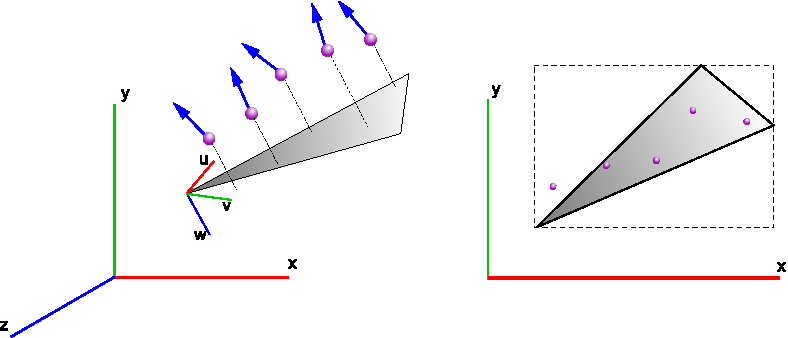
\includegraphics[height=40mm]{images/example_figure.pdf}
\captionfonts
\caption[This is a figure]{This is an example figure.  This graphic was drawn in InkScape (http://www.inkscape.org/), a free vector drawing application.  Figures can be exported from InkScape as PDF images or as EPS (depending upon if you want LaTeX to generate a PDF or a PostScript document.)}
\label{fig:inkscape-example}
\end{center}
\end{figure}



\chapter{Previous Work}
\label{previous-work}

LaTeX is a document markup language and document preparation system for the TeX typesetting program.

It is widely used by mathematicians, scientists, philosophers, engineers, and scholars in academia and the commercial world, and by others as a primary or intermediate format (e.g. translating DocBook and other XML-based formats to PDF) because of the quality of typesetting achievable by TeX. It offers programmable desktop publishing features and extensive facilities for automating most aspects of typesetting and desktop publishing, including numbering and cross-referencing, tables and figures, page layout and bibliographies.

LaTeX is intended to provide a high-level language to access the power of TeX. LaTeX essentially comprises a collection of TeX macros, and a program to process LaTeX documents. Since TeX's formatting commands are very low-level, it is usually much simpler for end-users to use LaTeX.

LaTeX was originally written in 1984 by Leslie Lamport at SRI International and has become the dominant method for using TeX�few people write in plain TeX anymore.

LaTeX is based on the idea that authors should be able to focus on the meaning of what they are writing, without being distracted by the visual presentation of the information. In preparing a LaTeX document, the author specifies the logical structure using familiar concepts such as chapter, section, table, figure, etc., and lets the LaTeX system worry about the presentation of these structures. It therefore encourages the separation of layout from content, while still allowing manual typesetting adjustments where needed. This is similar to the mechanism by which many word processors allow styles to be defined globally for an entire document, or the CSS mechanism used by HTML.

\section{This is a new section}
\label{a-new-section}

LaTeX is a document markup language and document preparation system for the TeX typesetting program.

It is widely used by mathematicians, scientists, philosophers, engineers, and scholars in academia and the commercial world, and by others as a primary or intermediate format (e.g. translating DocBook and other XML-based formats to PDF) because of the quality of typesetting achievable by TeX. It offers programmable desktop publishing features and extensive facilities for automating most aspects of typesetting and desktop publishing, including numbering and cross-referencing, tables and figures, page layout and bibliographies.

LaTeX is intended to provide a high-level language to access the power of TeX. LaTeX essentially comprises a collection of TeX macros, and a program to process LaTeX documents. Since TeX's formatting commands are very low-level, it is usually much simpler for end-users to use LaTeX.

\begin{figure}
\begin{center}
\[
\left[\begin{array}{ccc}
u_{x} & u_{y} & u_{z}\\
v_{x} & v_{y} & v_{z}\\
w_{x} & w_{y} & w_{z}\end{array}\right]\left[\begin{array}{c}
p_{x}\\
p_{y}\\
p_{z}\end{array}\right]=\left[\begin{array}{c}
p_{x}^{\prime}\\
p_{y}^{\prime}\\
p_{z}^{\prime}\end{array}\right]\]
\captionfonts
\caption[A matrix equation]{This is a sample matrix equation.}
\label{eqn:example}
\end{center}
\end{figure}


LaTeX was originally written in 1984 by Leslie Lamport at SRI International and has become the dominant method for using TeX�few people write in plain TeX anymore.

LaTeX is based on the idea that authors should be able to focus on the meaning of what they are writing, without being distracted by the visual presentation of the information. In preparing a LaTeX document, the author specifies the logical structure using familiar concepts such as chapter, section, table, figure, etc., and lets the LaTeX system worry about the presentation of these structures. It therefore encourages the separation of layout from content, while still allowing manual typesetting adjustments where needed. This is similar to the mechanism by which many word processors allow styles to be defined globally for an entire document, or the CSS mechanism used by HTML.


\begin{enumerate}
\item Here is a list item.
\begin{enumerate}
\item Here is a sub list item.
\begin{enumerate}
\item Here is a sub sub list item.

\end{enumerate}
\end{enumerate}
\end{enumerate}



\chapter{Results}
\label{results}

Here is the results section.

LaTeX is a document markup language and document preparation system for the TeX typesetting program.

It is widely used by mathematicians, scientists, philosophers, engineers, and scholars in academia and the commercial world, and by others as a primary or intermediate format (e.g. translating DocBook and other XML-based formats to PDF) because of the quality of typesetting achievable by TeX. It offers programmable desktop publishing features and extensive facilities for automating most aspects of typesetting and desktop publishing, including numbering and cross-referencing, tables and figures, page layout and bibliographies.

LaTeX is intended to provide a high-level language to access the power of TeX. LaTeX essentially comprises a collection of TeX macros, and a program to process LaTeX documents. Since TeX's formatting commands are very low-level, it is usually much simpler for end-users to use LaTeX.

LaTeX was originally written in 1984 by Leslie Lamport at SRI International and has become the dominant method for using TeX�few people write in plain TeX anymore.

LaTeX is based on the idea that authors should be able to focus on the meaning of what they are writing, without being distracted by the visual presentation of the information. In preparing a LaTeX document, the author specifies the logical structure using familiar concepts such as chapter, section, table, figure, etc., and lets the LaTeX system worry about the presentation of these structures. It therefore encourages the separation of layout from content, while still allowing manual typesetting adjustments where needed. This is similar to the mechanism by which many word processors allow styles to be defined globally for an entire document, or the CSS mechanism used by HTML.

LaTeX can be arbitrarily extended by using the underlying macro language to develop custom formats. Such macros are often collected into packages which are available to address special formatting issues such as complicated mathematical content or graphics. In addition, there are numerous commercial implementations of the entire TeX system, including LaTeX, to which vendors may add extra features like additional typefaces and telephone support. LyX is a free visual document processor that uses LaTeX for a back-end. TeXmacs is a free, WYSIWYG editor with similar functionalities as LaTeX, but a different typesetting engine.

A number of popular commercial desktop publishing systems use modified versions of the original TeX typesetting engine. The recent rise in popularity of XML systems and the demand for large-scale batch production of publication-quality typesetting from such sources has seen a steady increase in the use of LaTeX.


\begin{table}
\begin{center}

\begin{tabular}{|c|c|c|c|c|c|c|}
\hline 
&
\multicolumn{2}{c|}{Some Data}&
&
\multicolumn{2}{c|}{Some More Data}&
\tabularnewline
\hline
\hline 
&  Hi-Res&  Lo-Res&  Reduction&  Hi-Res&  Lo-Res&  Speedup
\tabularnewline
\hline 
Row Data A &  225,467&  43,850&  80.6\%&  360&  90&  4.0
\tabularnewline
\hline 
Row Data B &  225,467&  16,388&  92.7\%&  360&  26&  13.8
\tabularnewline
\hline 
\end{tabular}


\captionfonts
\caption[Performance data]{Here is some performance data for the system.}
\label{table:performance}
\end{center}
\end{table}


LaTeX is a document markup language and document preparation system for the TeX typesetting program.

It is widely used by mathematicians, scientists, philosophers, engineers, and scholars in academia and the commercial world, and by others as a primary or intermediate format (e.g. translating DocBook and other XML-based formats to PDF) because of the quality of typesetting achievable by TeX. It offers programmable desktop publishing features and extensive facilities for automating most aspects of typesetting and desktop publishing, including numbering and cross-referencing, tables and figures, page layout and bibliographies.

LaTeX is intended to provide a high-level language to access the power of TeX. LaTeX essentially comprises a collection of TeX macros, and a program to process LaTeX documents. Since TeX's formatting commands are very low-level, it is usually much simpler for end-users to use LaTeX.

LaTeX was originally written in 1984 by Leslie Lamport at SRI International and has become the dominant method for using TeX�few people write in plain TeX anymore.

LaTeX is based on the idea that authors should be able to focus on the meaning of what they are writing, without being distracted by the visual presentation of the information. In preparing a LaTeX document, the author specifies the logical structure using familiar concepts such as chapter, section, table, figure, etc., and lets the LaTeX system worry about the presentation of these structures. It therefore encourages the separation of layout from content, while still allowing manual typesetting adjustments where needed. This is similar to the mechanism by which many word processors allow styles to be defined globally for an entire document, or the CSS mechanism used by HTML.

LaTeX can be arbitrarily extended by using the underlying macro language to develop custom formats. Such macros are often collected into packages which are available to address special formatting issues such as complicated mathematical content or graphics. In addition, there are numerous commercial implementations of the entire TeX system, including LaTeX, to which vendors may add extra features like additional typefaces and telephone support. LyX is a free visual document processor that uses LaTeX for a back-end. TeXmacs is a free, WYSIWYG editor with similar functionalities as LaTeX, but a different typesetting engine.

A number of popular commercial desktop publishing systems use modified versions of the original TeX typesetting engine. The recent rise in popularity of XML systems and the demand for large-scale batch production of publication-quality typesetting from such sources has seen a steady increase in the use of LaTeX.


% ------------- End main chapters ----------------------

\clearpage
\bibliography{bibliography}
\bibliographystyle{plain}
%\addcontentsline{toc}{chapter}{Bibliography}

\end{document}
